


\section{Perintah Navigasi}
Sebelum melakukan perintah navigasi pastikan kita memiliki tools Spyder, anaconda dan selenium. Lakukan instalasi selenium dengan cara ketik "pip install selenium" pada anaconda.

kemudian buka aplikasi Spyder dan masukkan program berikut ini :
\begin{verbatim}
from selenium import webdriver
opsi = webdriver.firefox.options.Options()
opsi.headless = False
binary = webdriver.firefox.firefox_binary.FirefoxBinary(
'C:\\Program Files\\Mozilla Firefox\\firefox.exe')
cap = webdriver.common.desired_capabilities.
DesiredCapabilities().FIREFOX
cap['marionette'] = True
browser=webdriver.Firefox(options=opsi,
capabilities=cap,firefox_binary=binary)
browser.get('https://tokoperhutani.com/')
\end{verbatim}

Penjelasan : 
\begin{enumerate}
	\item From selenium import webdriver Modul selenium webdriver mengimplementasikan kelas yang mendukung berbagai browser termasuk Firefox, Chrome, Internet Explorer, Safari, yang lain, dan RemoteWebDri	ver juga untuk menguji pada browser yang tersedia di mesin jarak jauh. Kita perlu mengimpor webdriver dari paket Selenium untuk menggunakan metode Selenium WebDriver.
	\item Opsi adalah kelas dalam paket webdriver selenium firefox. opts adalah turunan dari kelas Opsi yang dipakai untuk program.
	\item Headless, Python memperbarui instance Options, untuk menyimpan informasi "pengguna ini ingin memulai instance browser headless”.
	\item Webdriver.common.desiredcapabilities.DesiredCapabilities().FIREFOX.   sebagai titik awal untuk membuat objek kemampuan yang diinginkan untuk meminta driver web jarak jauh untuk terhubung ke server selenium.  
	\item Marionette adalah driver otomatisasi untuk mesin Gecko Mozilla.
	\item Browser.get metode akan menavigasi ke halaman yang diberikan oleh URL. WebDriver akan menunggu hingga halaman dimuat penuh (yaitu, "onload" telah diaktifkan) sebelum mengembalikan kontrol ke tes atau skrip.
\end{enumerate}

Setelah anda membuat Tambahan Codingan  seperti diatas untuk merunning program anda tekan run pada bar diatas. Saat kotak yang ditandai pada gambar dibawah, berwarna merah artinya proses running program tersebut masih berjalan. Setelah program di run akan otomatis membuka Mozila Firefox dan akan langsung membuka website tokoperhutani secara otomatis.

\begin{figure}[ht!]
	\centering
	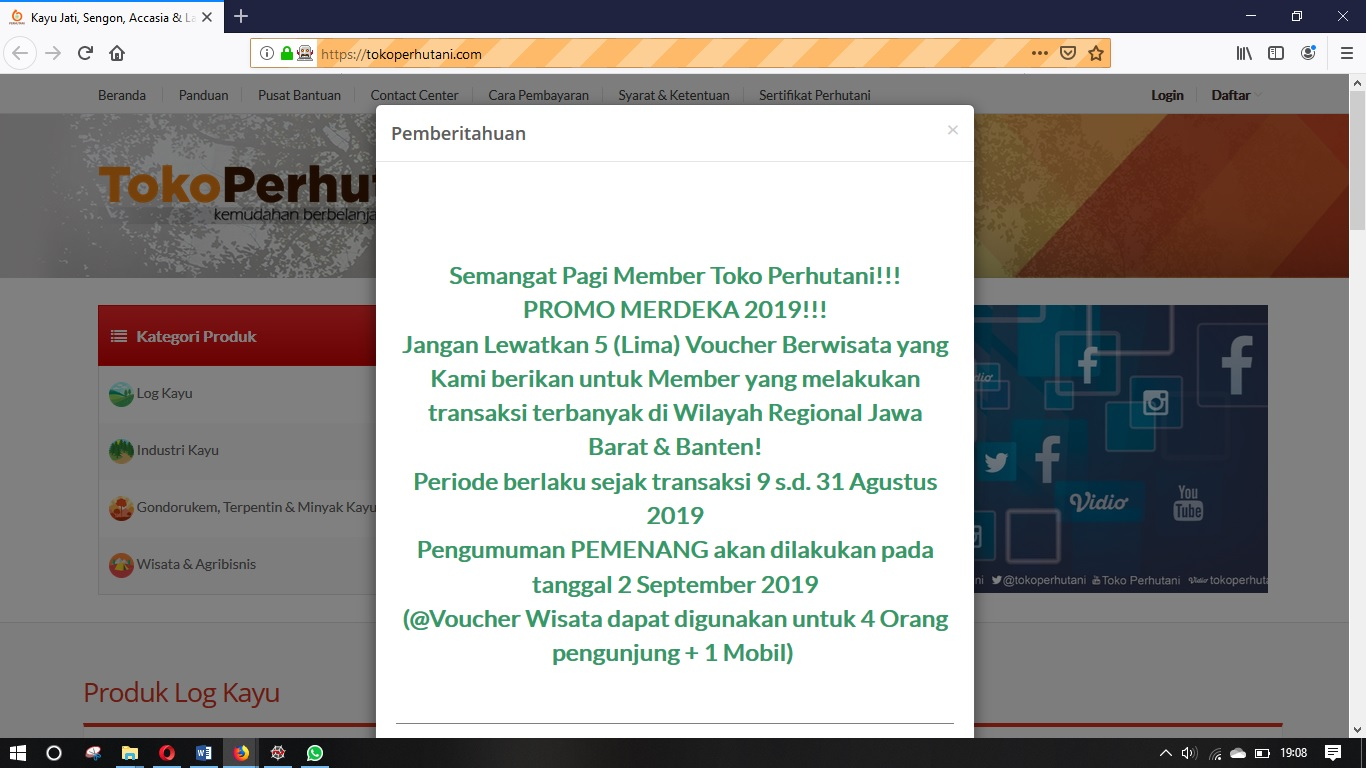
\includegraphics[scale=0.3]{figures/1x}
	\caption{Navigator Pada Menu Beranda}
\end{figure}

Masukkan code berikut untuk test navigator pada menu Cara Pembayaran:

\begin{verbatim}
pembayaran= browser.get('https://tokoperhutani.com/
article/static_art/cara-pembayaran')
\end{verbatim}

Hasilnya  di Mozilla Akan mucul seperti ini :
\begin{figure}[h]
	\centering
	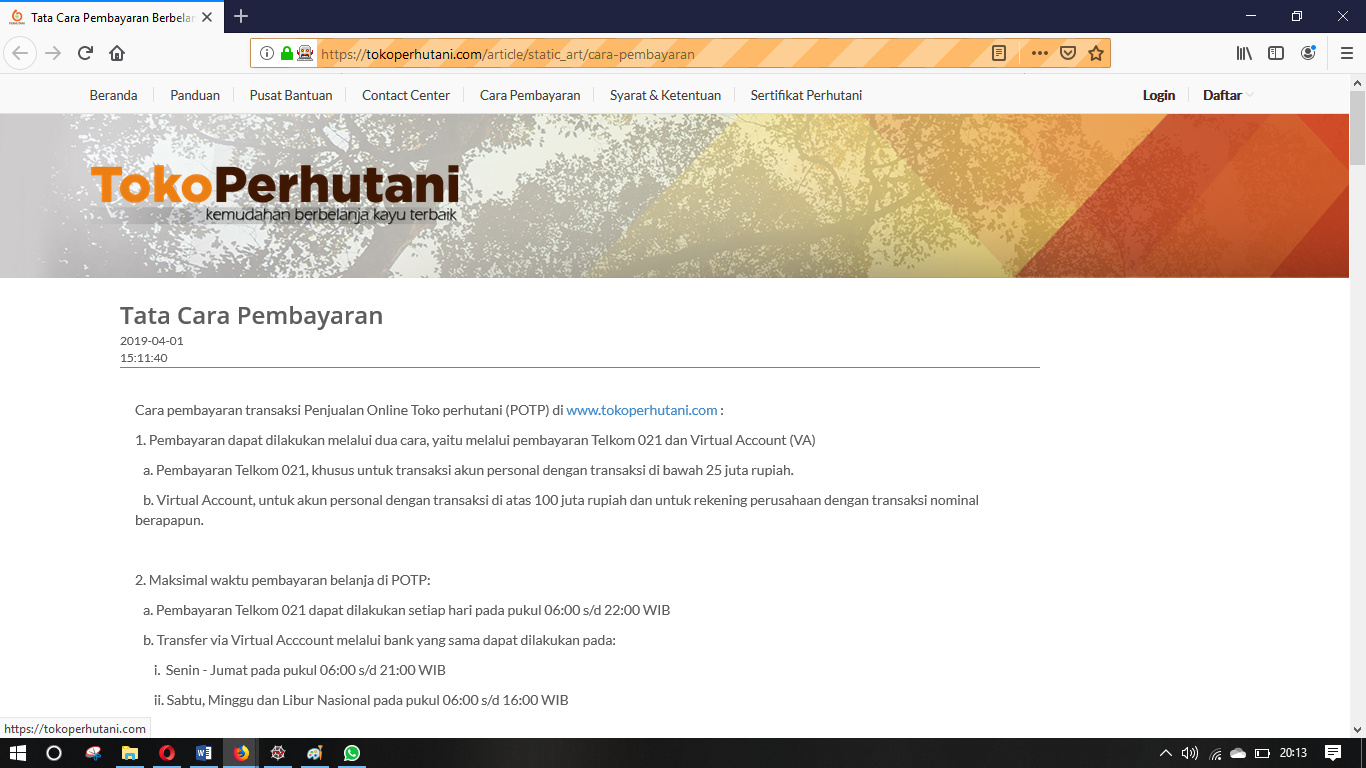
\includegraphics[scale=0.3]{figures/2}
	\caption{Tata Cara Pembayaran}
\end{figure}

Masukkan code berikut untuk test navigator pada menu Sertifikat Perhutani :

\begin{verbatim}
sertperhutani= browser.get('https://tokoperhutani.com/
SertifikatPerhutani')
\end{verbatim}

Hasilnya  di Mozilla Akan mucul seperti ini :
\begin{figure}[h]
	\centering
	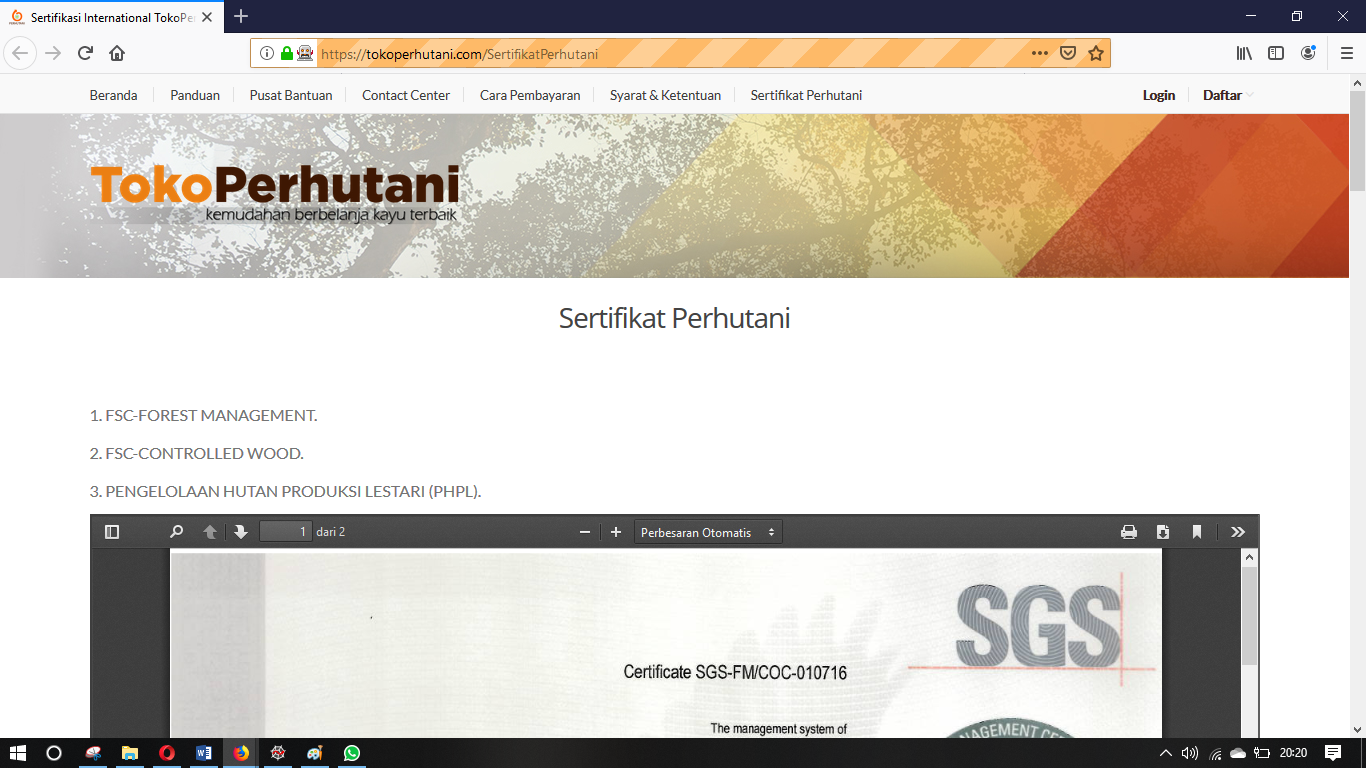
\includegraphics[scale=0.25]{figures/3}
	\caption{Navigator Pada Sertifikat Perhutani}
\end{figure}

Masukkan code berikut untuk test navigator pada menu  Panduan:
\begin{verbatim}
panduan = browser.get('https://tokoperhutani.com/
panduan')
\end{verbatim}

Hasilnya  di Mozilla Akan mucul seperti ini :
\begin{figure}[h]
	\centering
	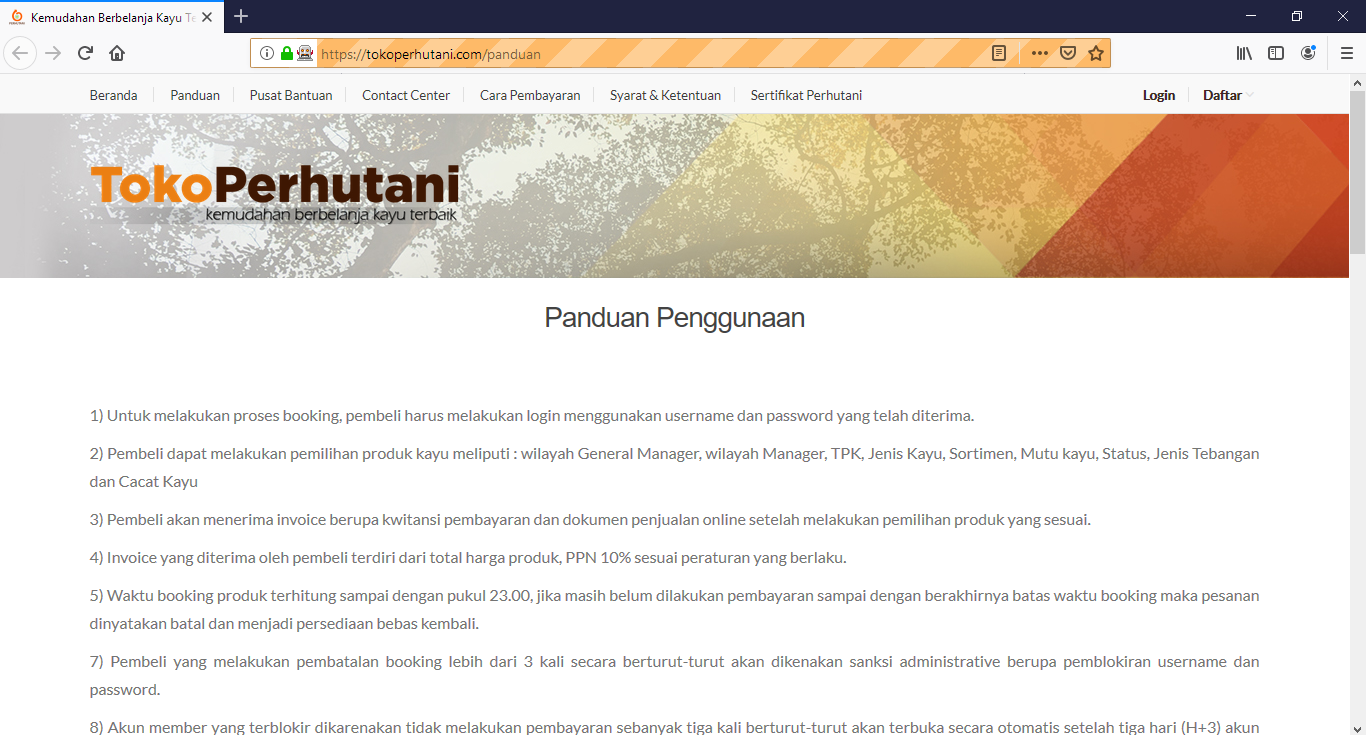
\includegraphics[scale=0.28]{figures/1hasil.PNG}
	\caption{Navigator Pada Panduan}
\end{figure}

Masukkan code berikut untuk test navigator pada menu  Pusat bantuan:
\begin{verbatim}
bantuan = browser.get('https://tokoperhutani.com/
faqs')
\end{verbatim}

Hasilnya  di Mozilla Akan mucul seperti ini :
\begin{figure}[h]
	\centering
	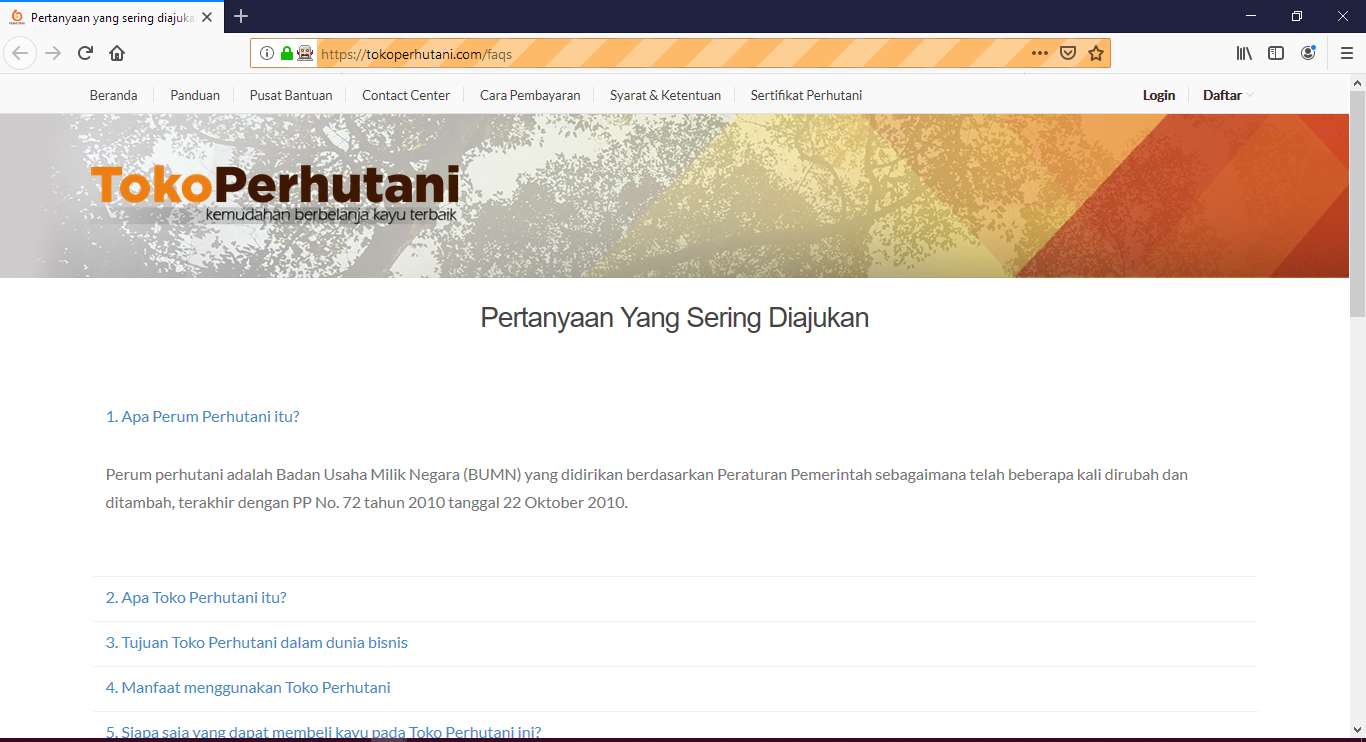
\includegraphics[scale=0.3]{figures/2hasil.PNG}
	\caption{Navigator Pada Pusat Bantuan}
\end{figure}

Masukkan code berikut untuk test navigator pada menu  Alamat kantor:
\begin{verbatim}
alamat = browser.get('https://tokoperhutani.com/
article/detil/alamat-kantor')
\end{verbatim}

Hasilnya  di Mozilla Akan mucul seperti ini :
\begin{figure}[h]
	\centering
	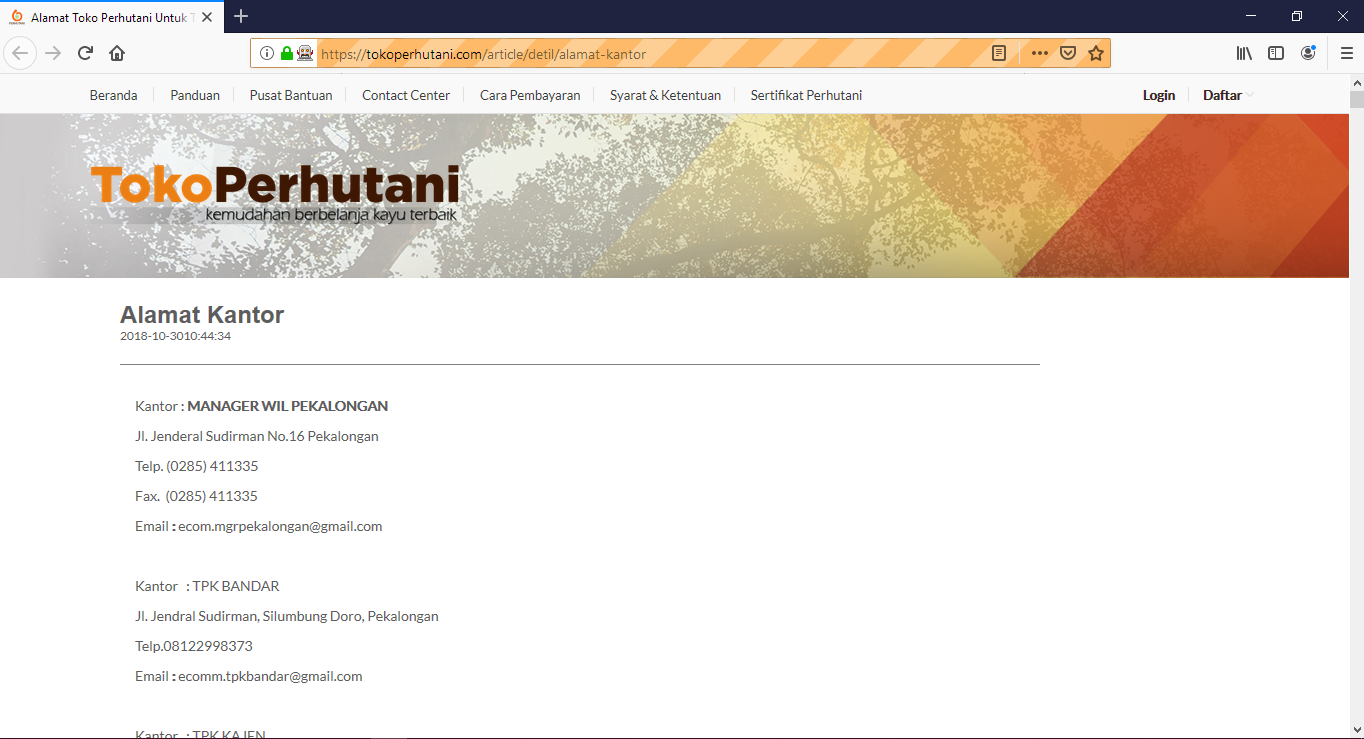
\includegraphics[scale=0.3]{figures/3hasil.PNG}
	\caption{Navigator Pada Alamat Kantor}
\end{figure}
\\

Masukkan code berikut untuk test navigator ke halaman panduan Registrasi:
\begin{verbatim}
browser.find_element_by_link_text('Registrasi')
.click()
\end{verbatim}

Hasilnya  di Google Chrome Akan mucul seperti ini :
\begin{figure}[h]
	\centering
	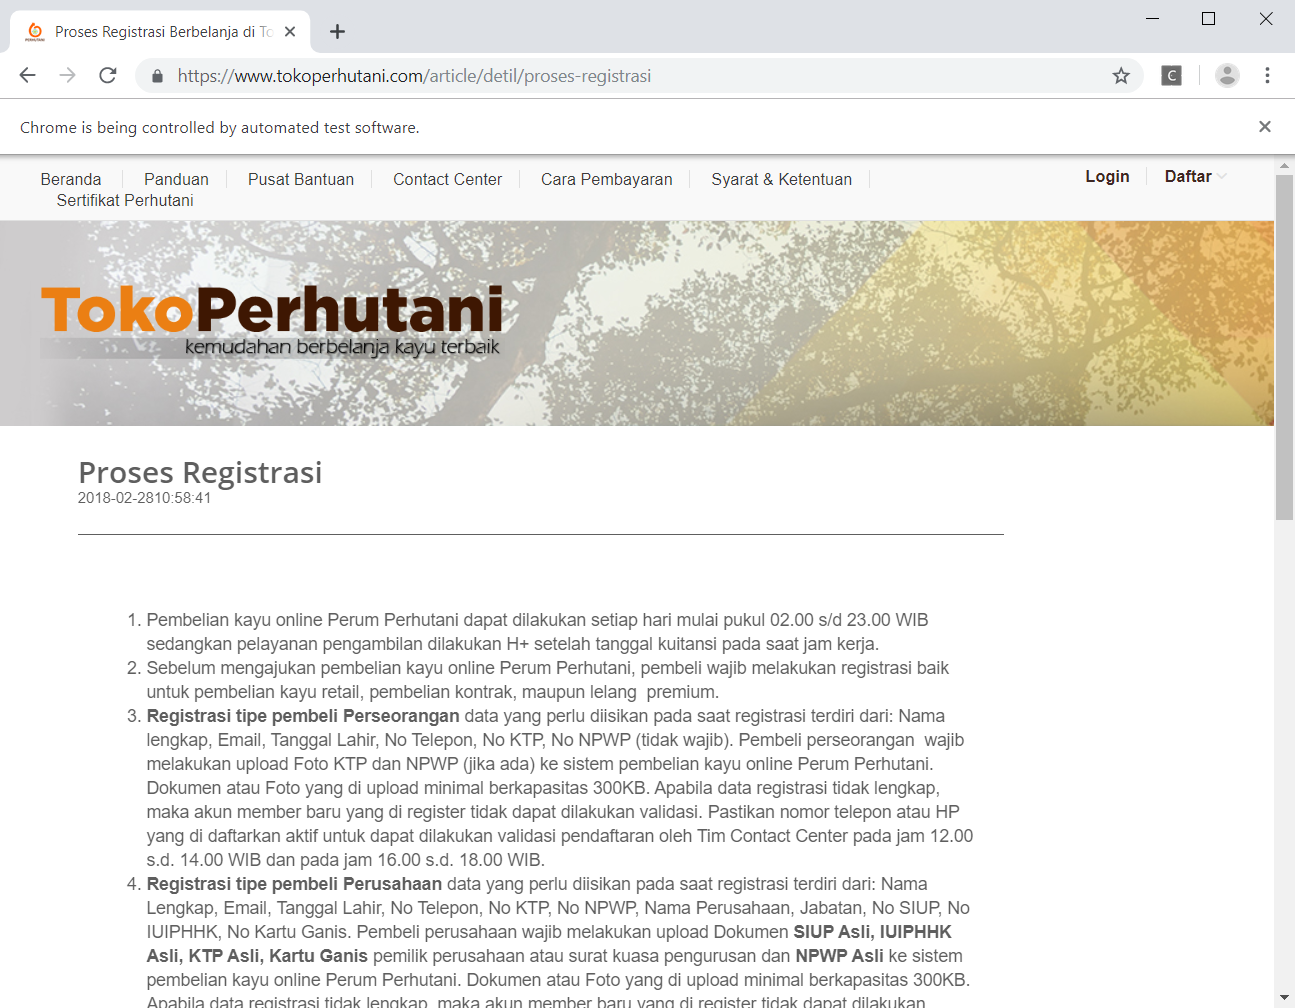
\includegraphics[scale=0.24]{figures/1pdregis}
	\caption{Halaman Panduan Registrasi}
\end{figure}

Masukkan code berikut untuk test menampilkan pilihan pendaftaran:
\begin{verbatim}
browser.find_element_by_link_text('Daftar')
.click()
\end{verbatim}

Hasilnya  di Google Chrome Akan mucul seperti ini :
\begin{figure}[h]
	\centering
	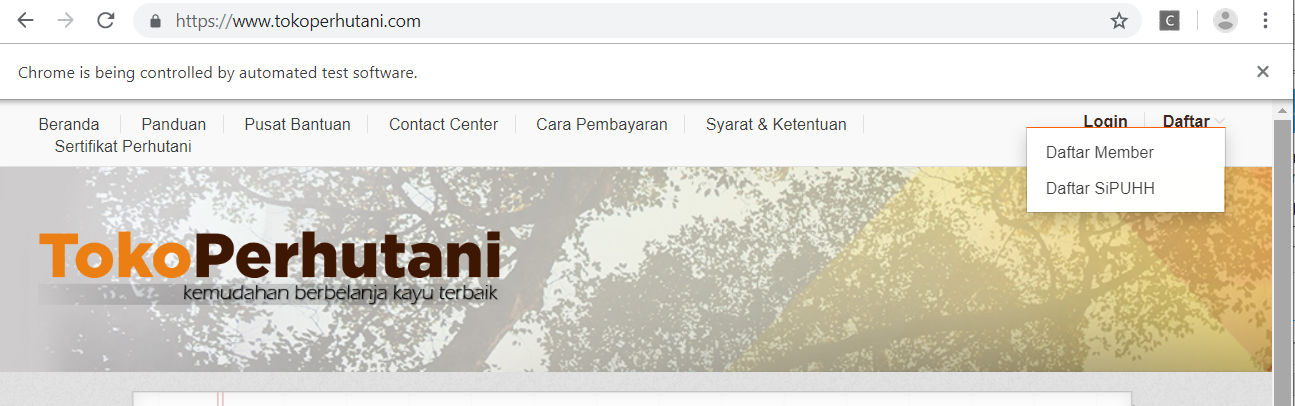
\includegraphics[scale=0.42]{figures/2daftar}
	\caption{Tombol navigasi Daftar}
\end{figure}

Masukkan code berikut untuk test memilih Daftar member:
\begin{verbatim}
browser.find_element_by_link_text('Daftar Member')
.click()
\end{verbatim}

Hasilnya  di Google Chrome Akan mucul seperti ini :
\begin{figure}[h]
	\centering
	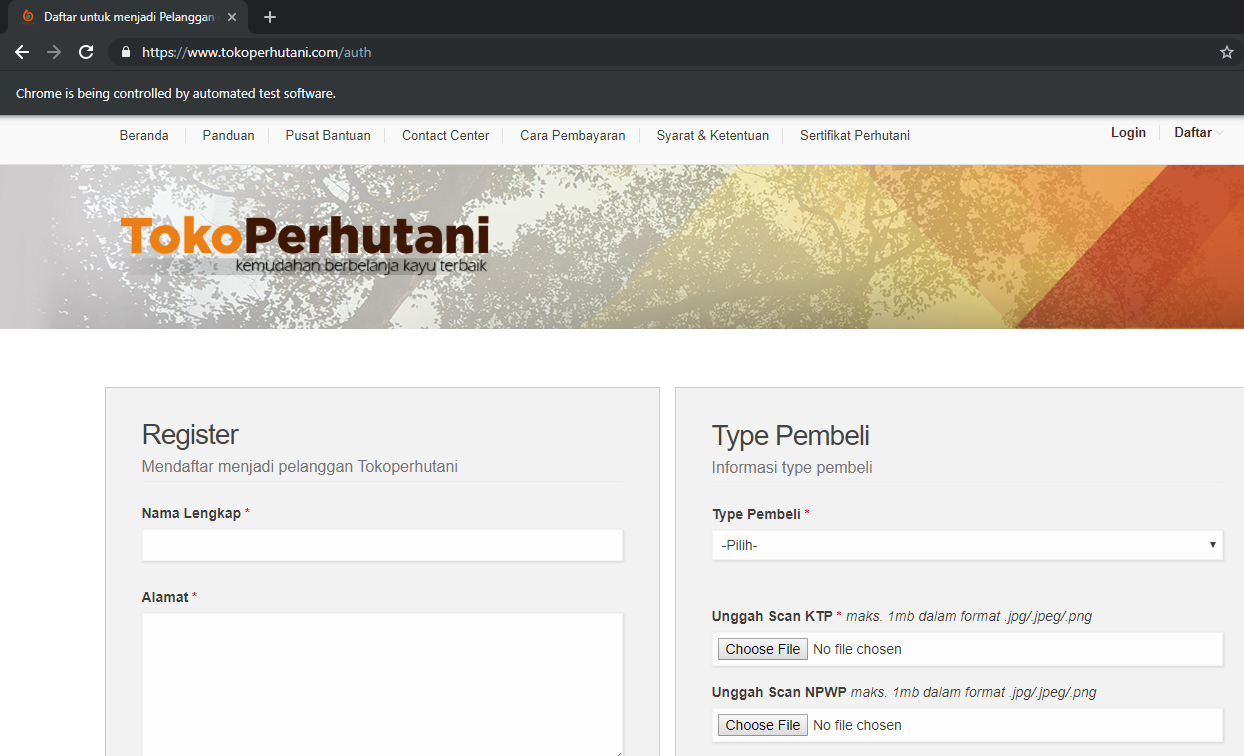
\includegraphics[scale=0.37]{figures/3daftar}
	\caption{Halaman Daftar Member}
\end{figure}

Masukkan code berikut untuk test navigator ke halaman Contact Center:
\begin{verbatim}
browser.find_element_by_link_text('Contact Center')
.click()
\end{verbatim}

Hasilnya  di Google Chrome Akan mucul seperti ini :
\begin{figure}[h]
	\centering
	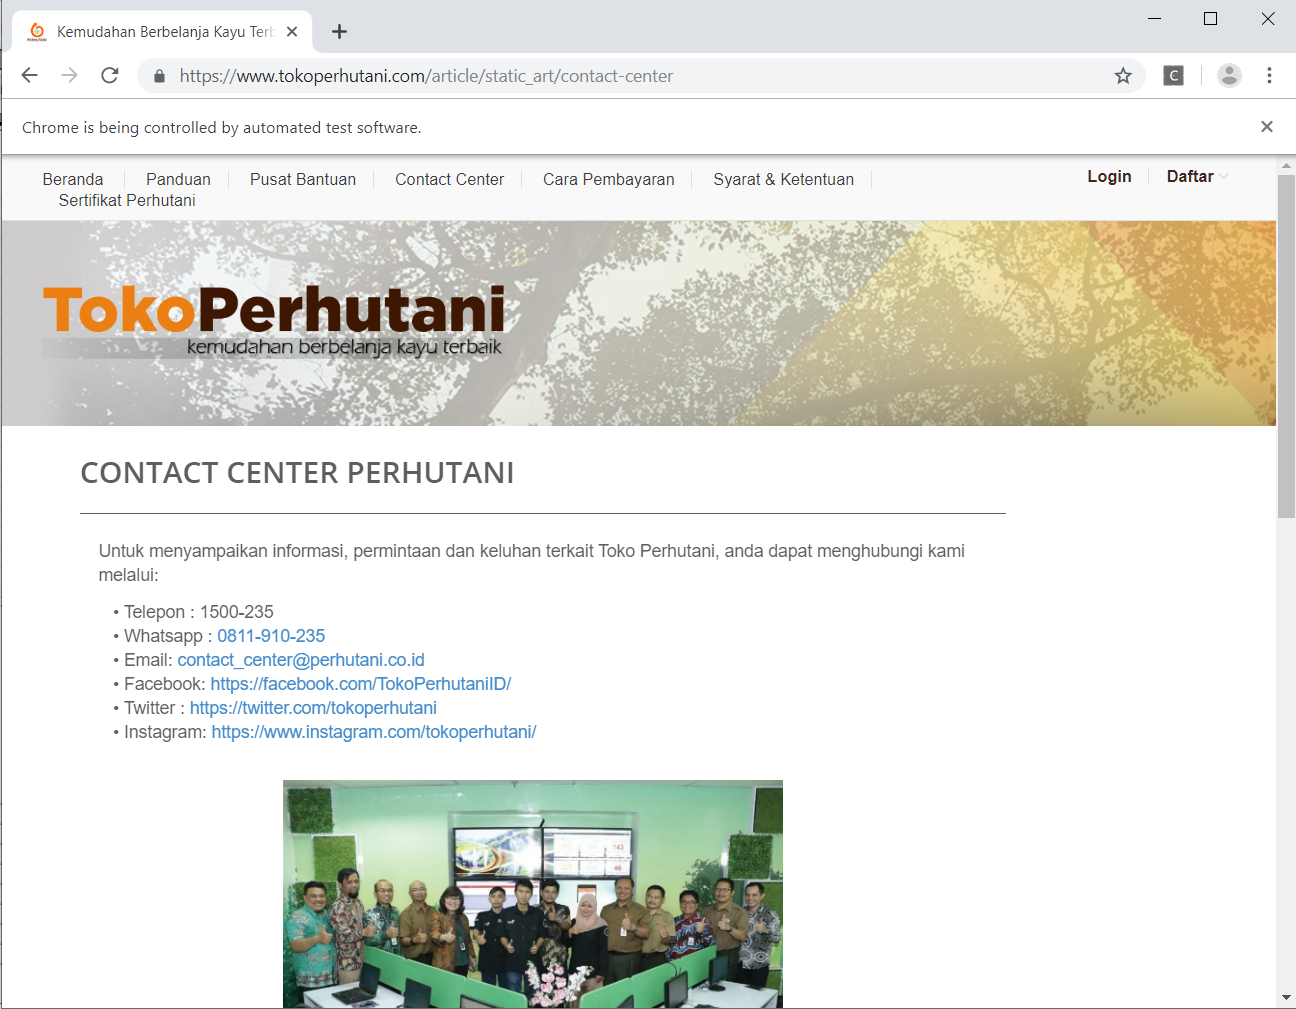
\includegraphics[scale=0.3]{figures/4kontak}
	\caption{Halaman Contact Center}
\end{figure}

Masukkan code berikut untuk test navigator pada menu Kayu Pinus:

\begin{verbatim}
KayuPinus = browser.get('https://tokoperhutani.com/
article/detil/kayu-pinus'
\end{verbatim}

Hasilnya  di Mozilla Akan mucul seperti ini :
\begin{figure}[h]
	\centering
	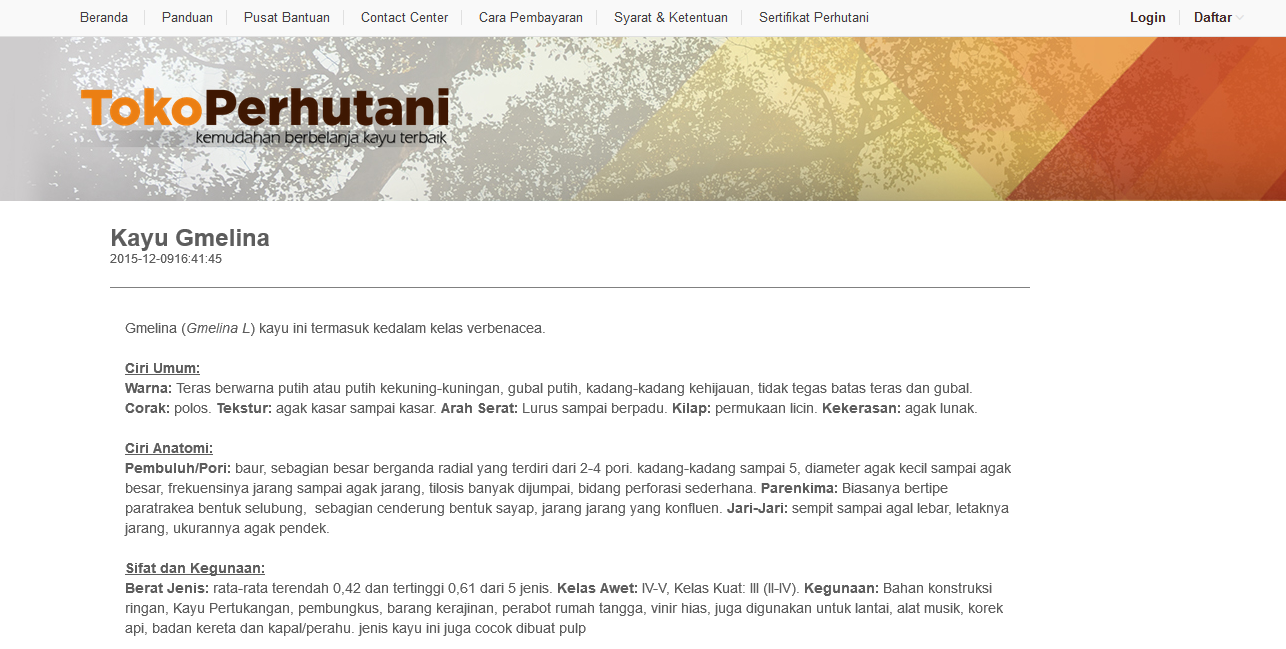
\includegraphics[scale=0.29]{figures/aa}
	\caption{Kayu Pinus}
\end{figure}

Masukkan code berikut untuk test navigator pada menu Kayu Gamelina :
\begin{verbatim}
KayuGmelina = browser.get('https://tokoperhutani
.com/article/detil/kayu-gmelina'
\end{verbatim}

Hasilnya  di Mozilla Akan mucul seperti ini :
\begin{figure}[h]
	\centering
	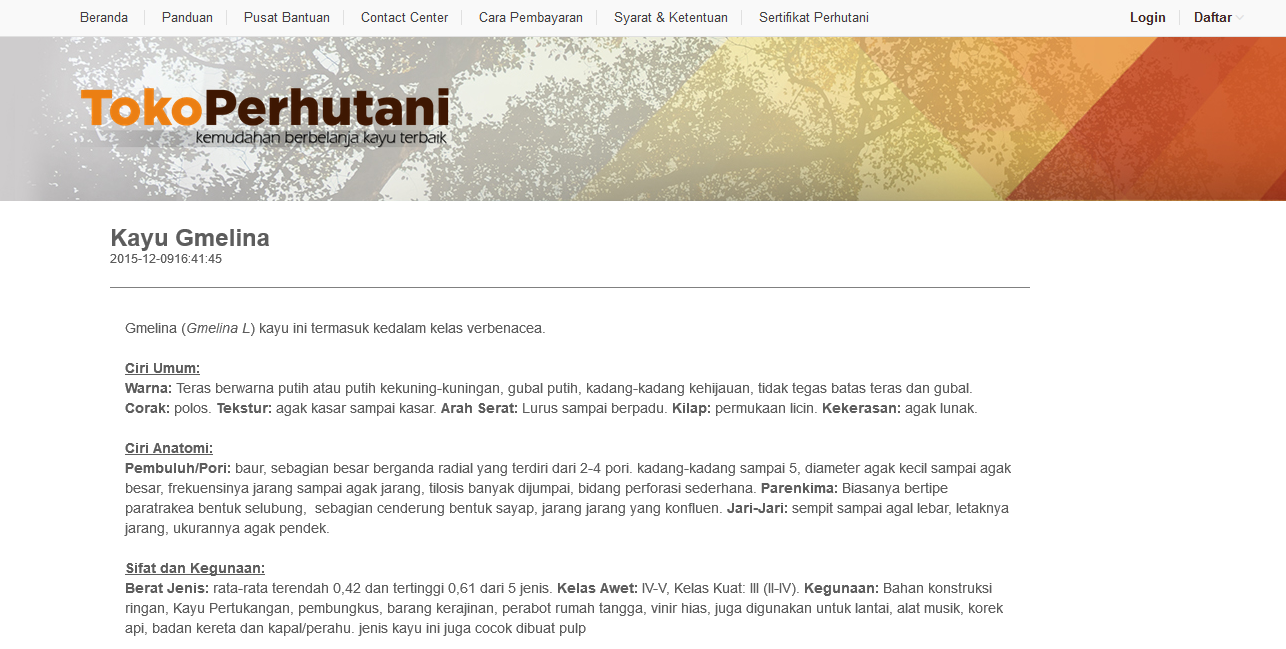
\includegraphics[scale=0.342]{figures/2kg}
	\caption{Kayu Gamelina}
\end{figure}

Masukkan code berikut untuk test navigator pada menu Kayu Sonokeling :
\begin{verbatim}
KayuSonokeling = browser.get('https://tokoperhu
tani.com/article/detil/kayu-sonokeling'
\end{verbatim}

Hasilnya  di Mozilla Akan mucul seperti ini :
\begin{figure}[h]
	\centering
	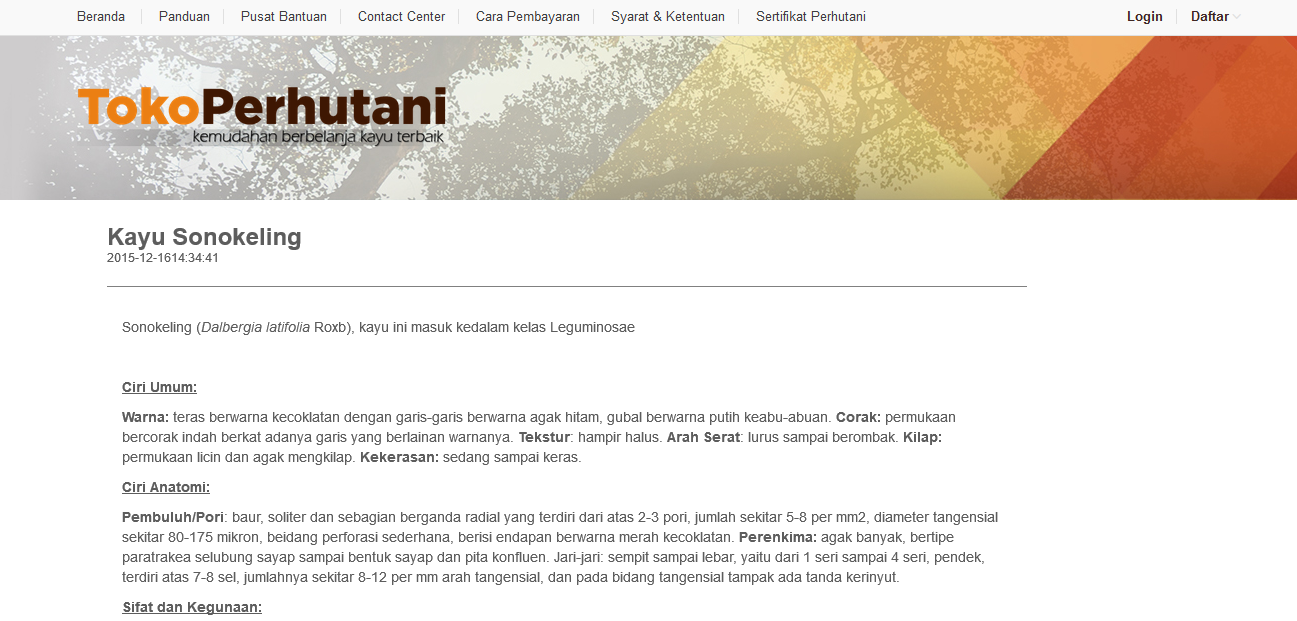
\includegraphics[scale=0.332]{figures/cc}
	\caption{Kayu Sonokeling}
\end{figure}

Masukkan code berikut untuk test navigator pada menu Kayu Pinus :
\begin{verbatim}
kayupinus = browser.get('https://www.tokoperhu
tani.com/article/detil/kayu-pinus')
\end{verbatim}

Hasilnya  di Mozilla Akan mucul seperti ini :
\begin{figure}[h]
	\centering
	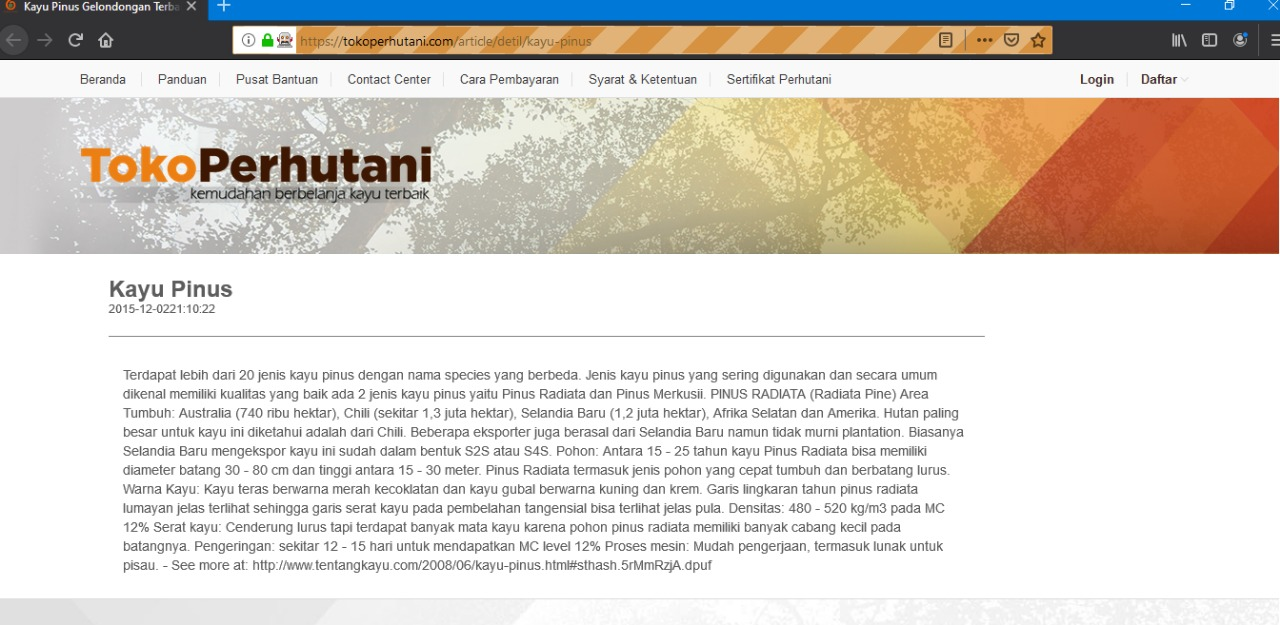
\includegraphics[scale=0.25]{figures/j1}
	\caption{Kayu Pinus}
\end{figure}

Masukkan code berikut untuk test navigator pada menu Kayu Gmelina :
\begin{verbatim}
kayugmelina  = browser.get('https://www.toko
perhutani.com/article/detil/kayu-gmelina')
\end{verbatim}

Hasilnya  di Mozilla Akan mucul seperti ini :
\begin{figure}[h]
	\centering
	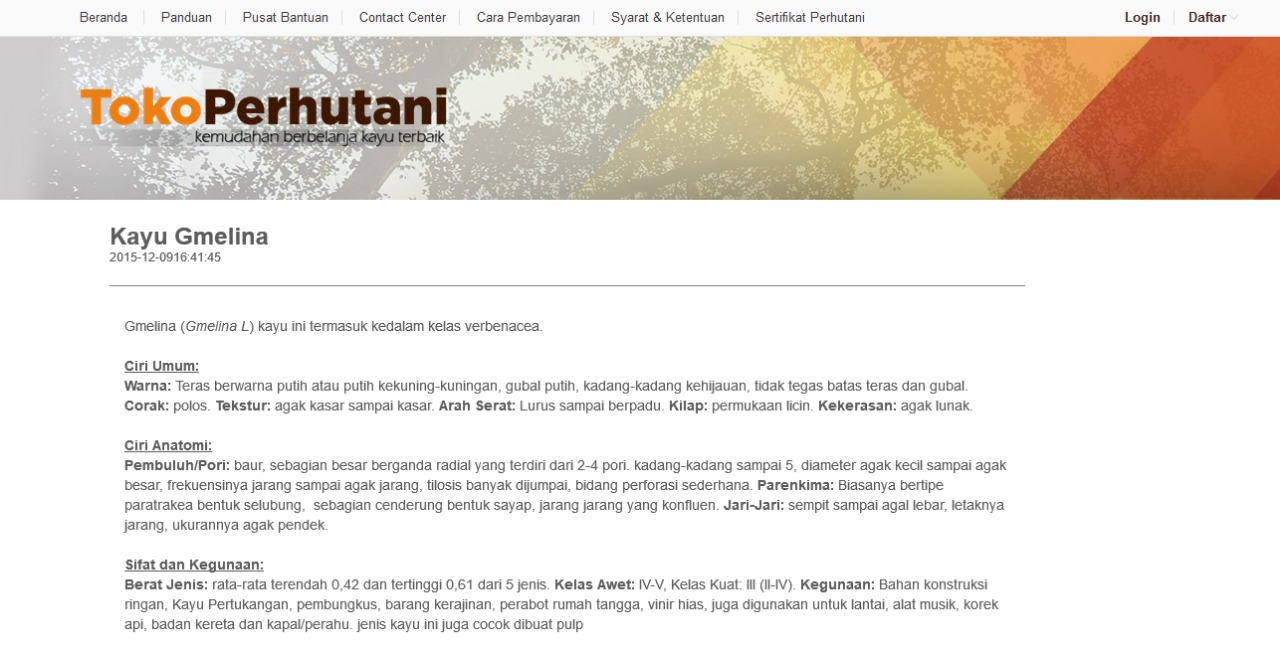
\includegraphics[scale=0.255]{figures/j2}
	\caption{Kayu Gmelina}
\end{figure}

Masukkan code berikut untuk test navigator pada menu Kayu Sonokeling :
\begin{verbatim}
kayusonokeling =  browser.get('www.tokoper
hutani.com/article/detil/kayu-sonokeling')
\end{verbatim}

Hasilnya  di Mozilla Akan mucul seperti ini :
\begin{figure}[h]
	\centering
	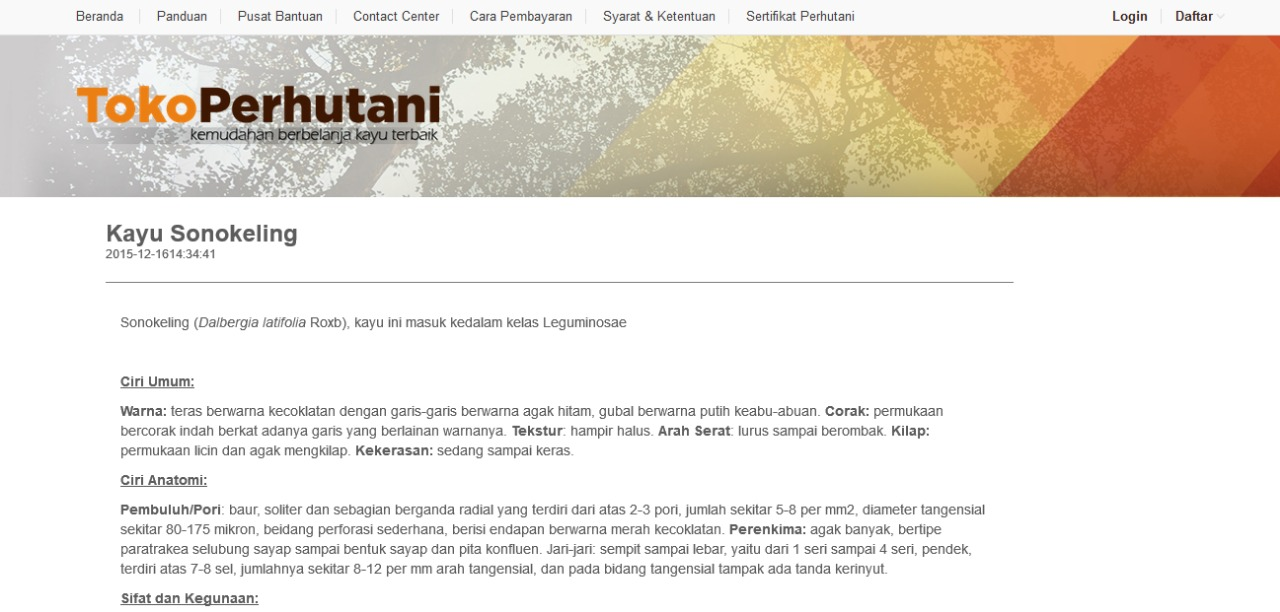
\includegraphics[scale=0.25]{figures/j3}
	\caption{Kayu Sonokeling}
\end{figure}

\newpage
\section{Pendaftaran Member}
Pada tutorial ini membutuhkan file gambar ktp untuk verivikasi data.

Masukan kode dibawah ini yang berfungsi untuk meng-import modul selenium dan time.
\begin{verbatim}
from selenium import webdriver
from time import sleep

browser = webdriver.Chrome()
web_pht = 'https://www.tokoperhutani.com/'

browser.get(web_pht)

browser.find_element_by_xpath('//*[@id="bannerModal"]/div/div/div[1]/button').click()

\end{verbatim}

Penjelasan:
\begin{enumerate}
	\item mengimport modul selenium dan time.
	\item lalu tahap selanjutnya membuka webdriver chrome / firefox dan membuka link web perhutani.
	\item karena di halaman landing page web toko perhutani terdapat modal yang menutupi halaman disini kita menutupnya.
\end{enumerate}


Hasilnya tampilan beranda awal website tokoperhutani:


\begin{figure}[h]
	\centering
	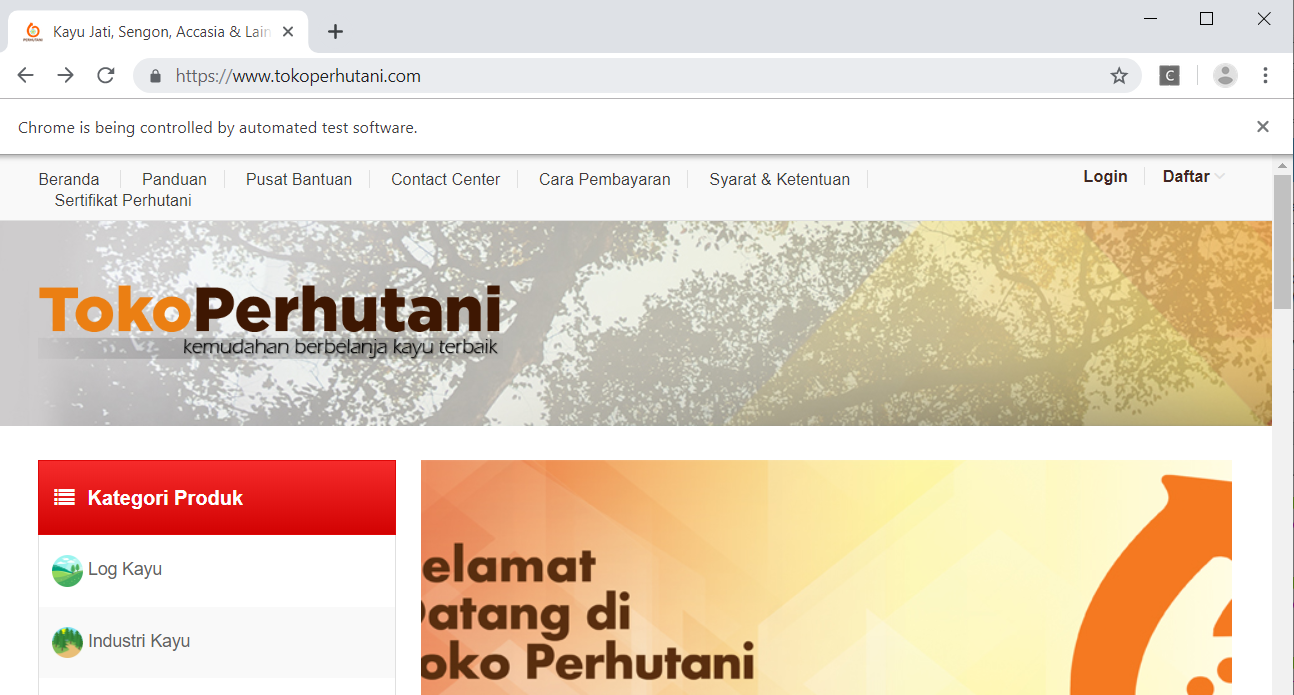
\includegraphics[scale=0.425]{figures/1home}
	\caption{Navigator Pada Menu Beranda}
\end{figure}
Masukkan code berikut untuk test masuk menu pendaftaran dengan menekan tombol daftar lalu memilih daftar member :
\begin{verbatim}
browser.find_element_by_link_text('Daftar').click()
sleep(1)
browser.find_element_by_link_text('Daftar Member').click()
\end{verbatim}

Hasilnya  di Google Chrome Akan mucul seperti ini :
\begin{figure}[h]
	\centering
	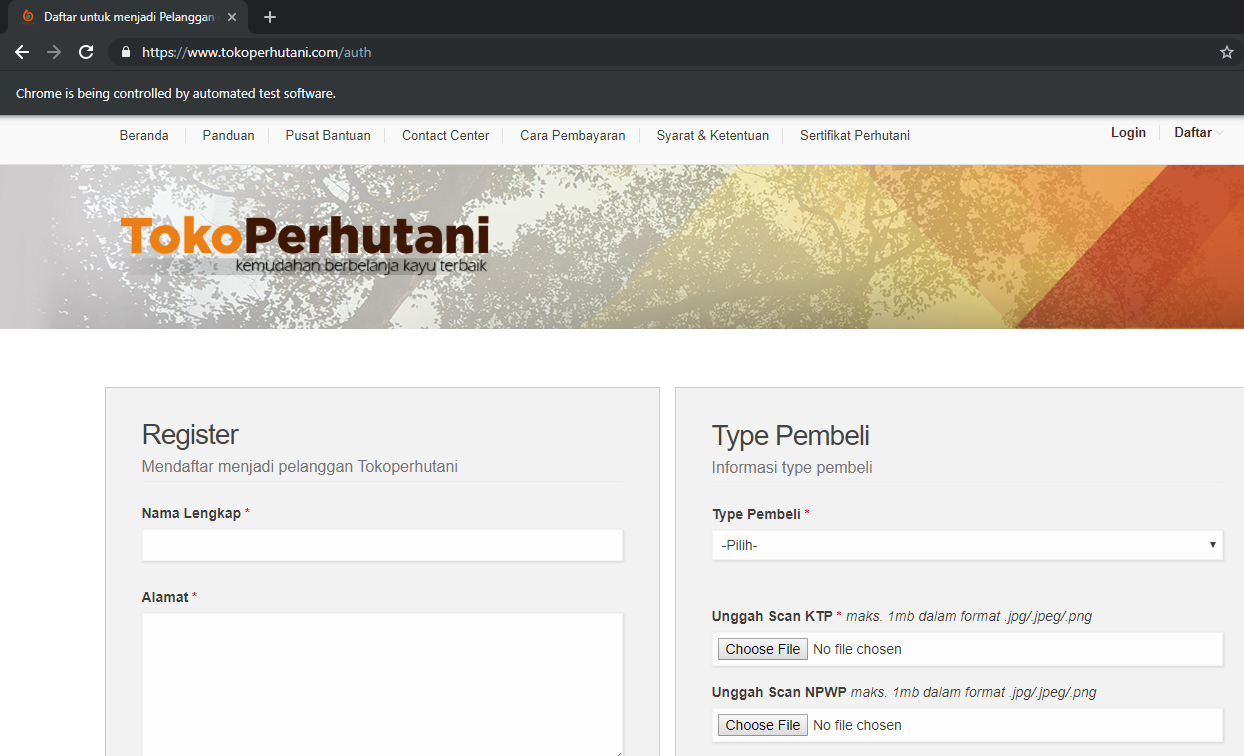
\includegraphics[scale=0.25]{figures/3daftar}
	\caption{Halaman Daftar}
\end{figure}

Masukkan code berikut untuk test mengisi form nama dan alamat :
\begin{verbatim}
browser.find_element_by_xpath('//*[@id="nama"]').send_keys('Kurnia dani')
browser.find_element_by_xpath('//*[@id="alamat"]').send_keys('jalan Sariasih no 2')
\end{verbatim}

Hasilnya akhir pada mozila firefox Akan mucul seperti ini:
\begin{figure}[h]
	\centering
	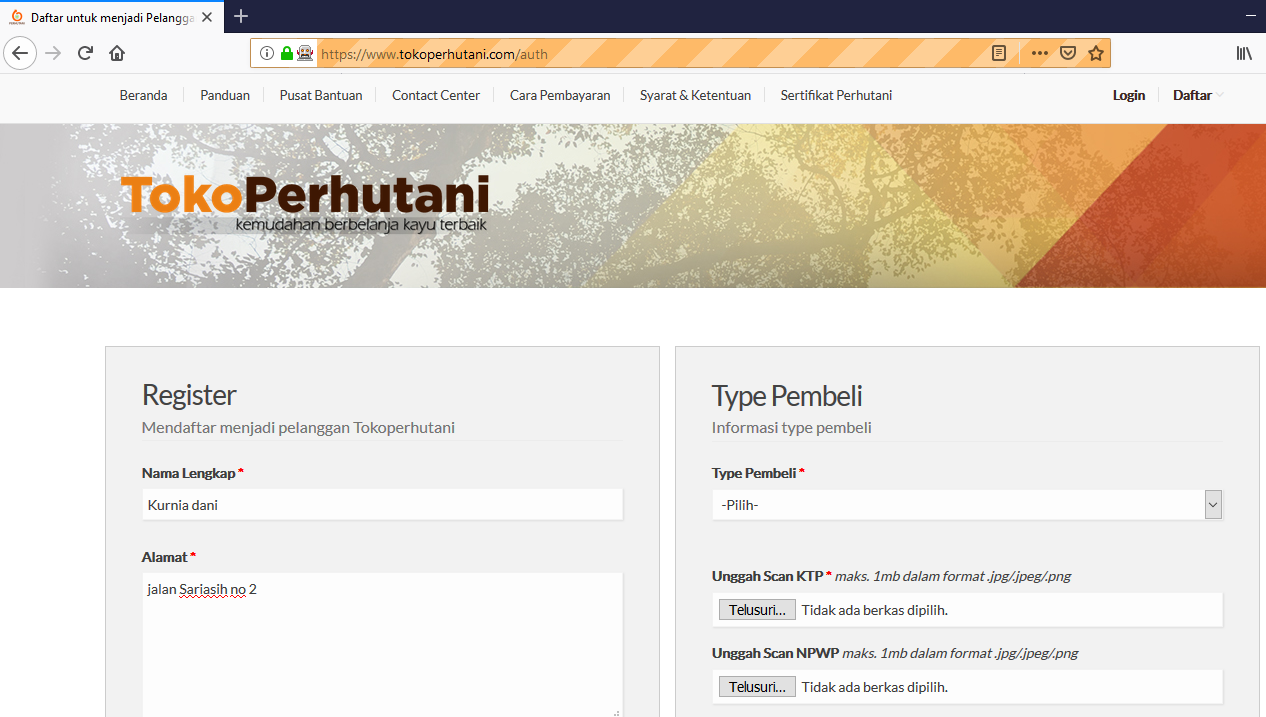
\includegraphics[scale=0.25]{figures/4daftar}
	\caption{Halaman Daftar}
\end{figure}


















\newpage
\section{Reset Password, Login Dan Menghubungi Contact Person di WA WA}
\subsection{Login}
Selanjutnya kita akan mencoba untuk melakukan login pada tool dengan selenium. 
Masukkan kode berikut untuk menampilkan form login:
\begin{verbatim}
content..browser.find_element_by_xpath('/html/body/div/
nav/div/div[2]/ul/li[1]/a/strong').click().
\end{verbatim}



Berikut hasil dari codingan di atas:
\begin{figure}[h]
	\centering
	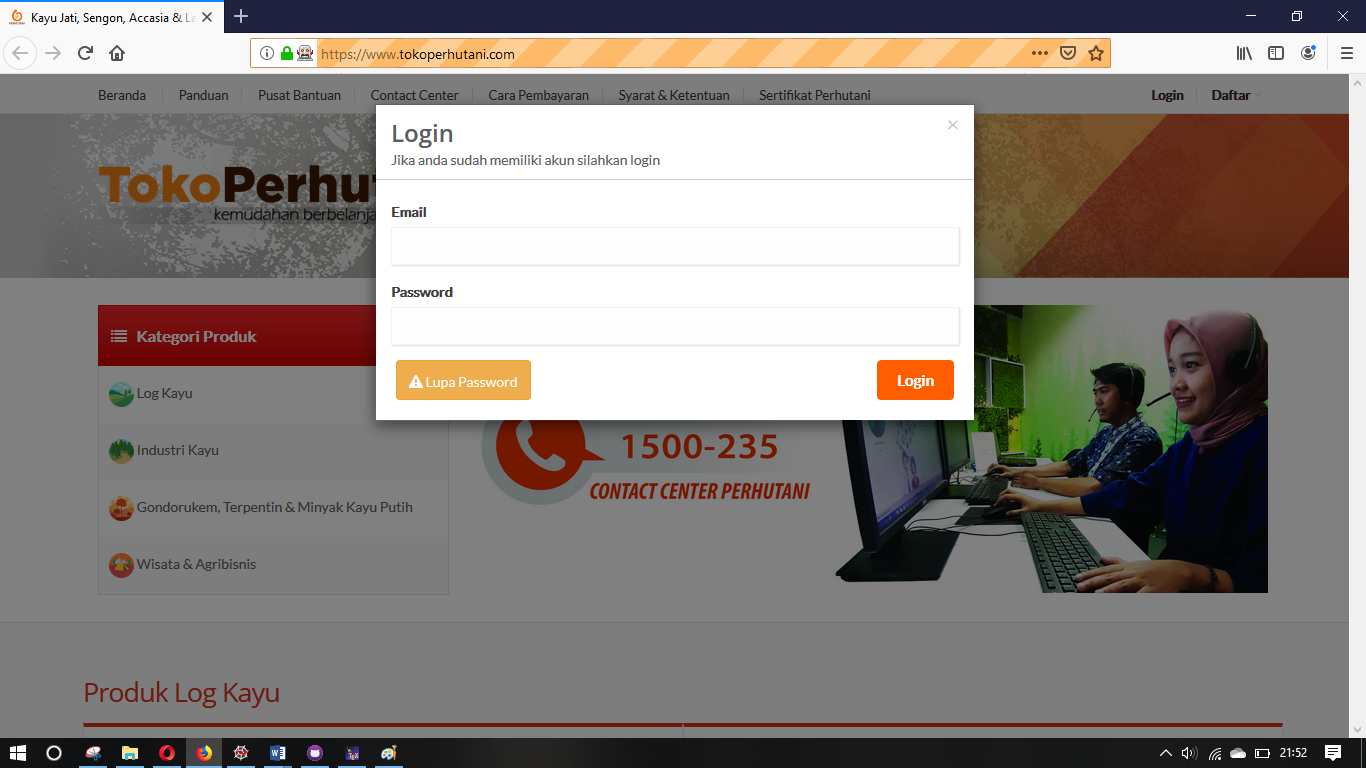
\includegraphics[scale=0.20]{figures/0login}
	\caption{Halaman Login}
\end{figure}

kemudian tambahkan kode berikut untuk memasukkan email, password dan tombol untuk mengclick login secara otomatis: 
\begin{verbatim}
browser.find_element_by_id('email').
send_keys('nsfthrn@gmail.com')

browser.find_element_by_id('password').
send_keys("C4CA2F")

browser.find_element_by_class_name('le-button').click() 
\end{verbatim}
\newpage
Kemudian akan muncul proses login seperti berikut:
\begin{figure}[h]
	\centering
	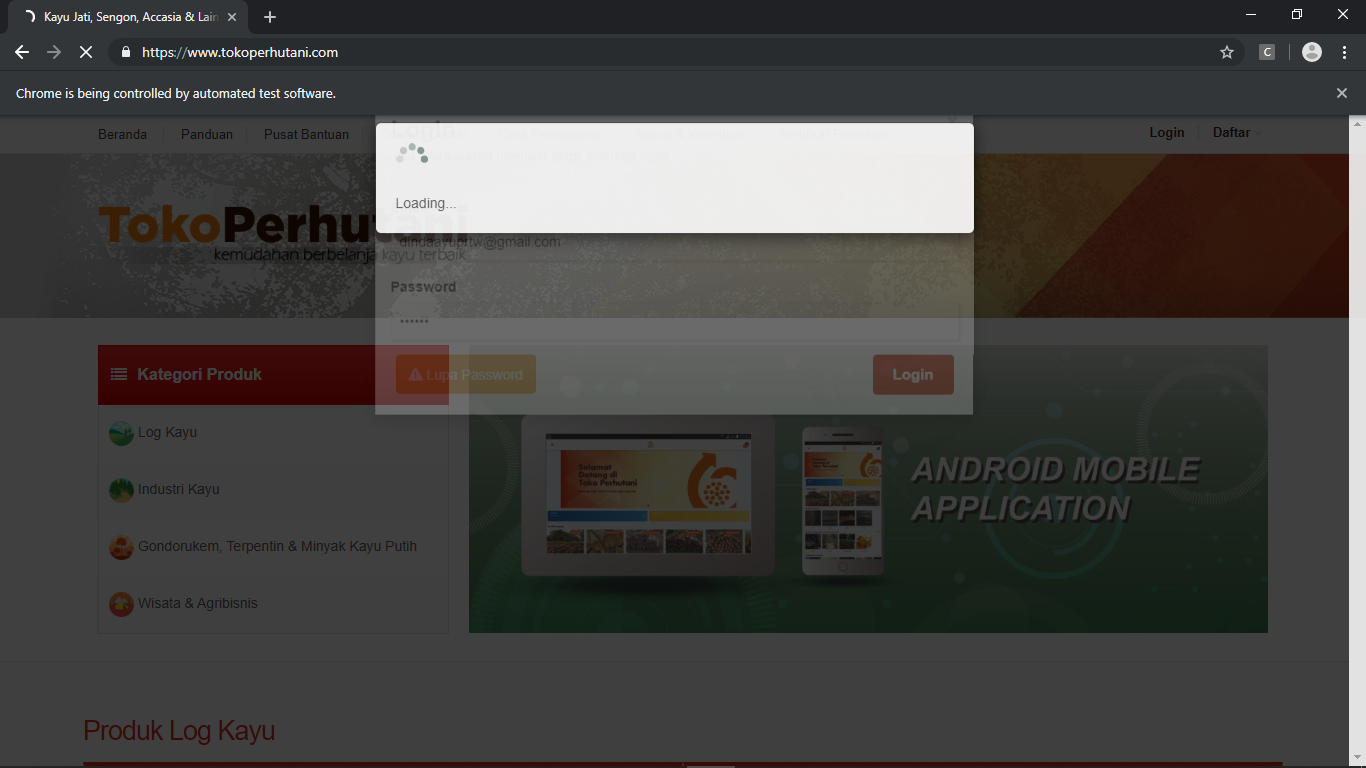
\includegraphics[scale=0.21]{figures/1login}
	\caption{Proses Login}
\end{figure}

Setelah proses loading selesai maka Login berhasil dan akan muncul tampilan seperti berikut:
\begin{figure}[h]
 	\centering
 	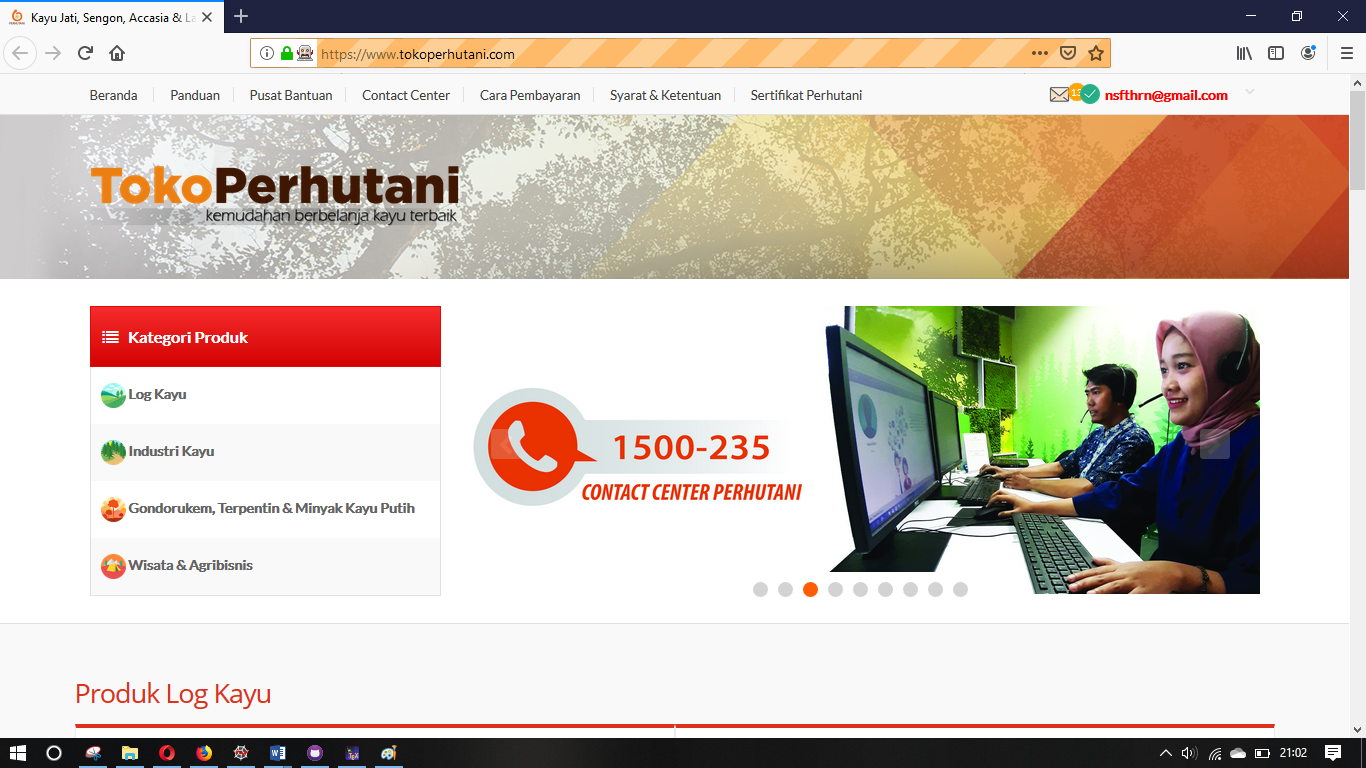
\includegraphics[scale=0.20]{figures/2login}
 	\caption{Login Berhasil}
\end{figure}



















































































































\newpage
\section{Cara Login Dan Melihat NIK KTP Pada Profil}
Kali ini kita akan membuat langkah-langkah untuk masuk ke akun tokoperhutani.com dan melihat nik KTP pada menu profil.  
\subsection{Tutorial Login}
Untuk login pada akun tokoperhutani.com masukkan kode berikut pada tool Spyder:
\begin{verbatim}
browser.find_element_by_xpath('/html/body/div
/nav/div/div[2]/ul/li[1]/a/strong').click()
browser.find_element_by_id('email').send_keys
('novinurinabb25@gmail.com')
browser.find_element_by_id('password').send_k
eys("86083F")
browser.find_element_by_class_name('le-button
').click()
\end{verbatim}

Penjelasan:
\begin{enumerate}
	\item Baris pertama untuk mengklik menu login agar form login terbuka.
	\item Baris Kedua untuk mengisikan email pada form login. 
	\item Baris Ketiga untuk mengisi password pada form login.
	\item Baris Keempat untuk mengklik tombol login agar bisa login ke akun yang di inputkan di email dan password.
\end{enumerate}

\newpage
\subsection{Mencari NIK KTP Pada Profile}
Untuk mencari dan menemukan NIK KTP pada profil, masukkan code berikut :
\begin{verbatim}
browser.find_element_by_xpath('/html/body/div/nav/div/div[2]
/ul/strong/li/a').click()
browser.find_element_by_link_text('Profile').click()
\end{verbatim}

Penjelasan:
\begin{enumerate}
	\item Baris Pertama untuk menampilkan menu pada bar
	\item Baris Kedua untuk meng-klik profil dan menampilkan data dan di dalamnya terdapat NIK
\end{enumerate}

Hasil dari menjalankan code baris ke 1:
\begin{figure}[h]
	\centering
	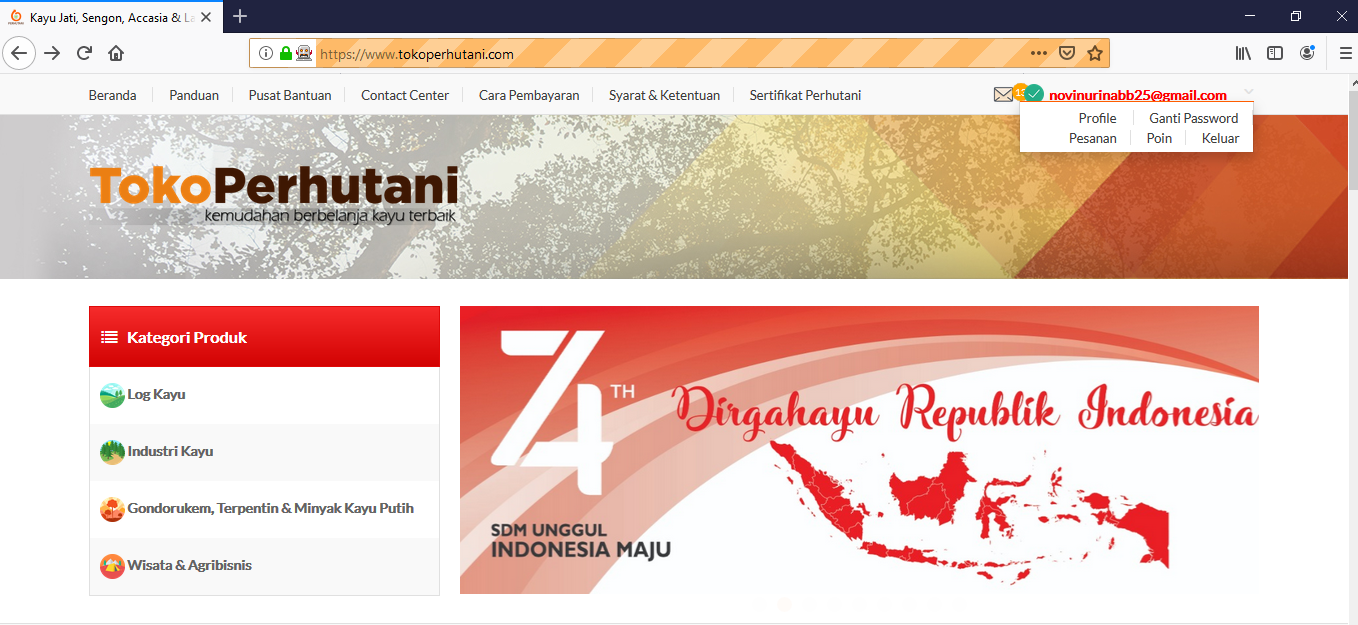
\includegraphics[scale=0.25]{figures/caripropil}
	\caption{Menampilkan Menu Bar Profil}
\end{figure}

Hasil menjalankan code baris ke 2:
\begin{figure}[h]
	\centering
	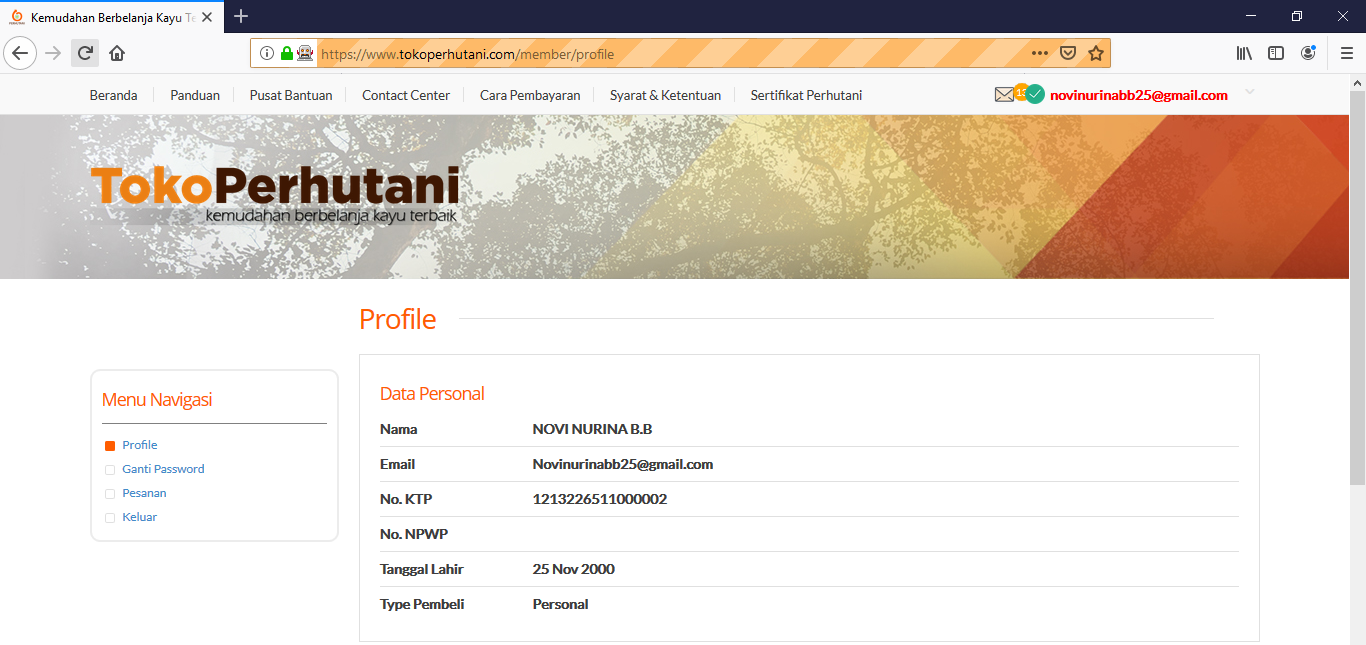
\includegraphics[scale=0.25]{figures/cari}
	\caption{Halaman Profil}
\end{figure}